\documentclass{article}
\usepackage[utf8]{inputenc}
\usepackage{fancyhdr}
\usepackage{graphicx}
\usepackage{geometry}
\usepackage{float}

% ---- Commands ------- %
\newcommand{\documentNumber}[1]{
    \LARGE  \textbf{ Kravspecifikation }
    \\
    \medskip
}
\newcommand{\documentVersion}[1]{
    \medskip
}
\newcommand{\documentTitle}[1]{
    \centerline{\rule{13cm}{0.4pt}}
    \bigskip \bigskip
    \LARGE \textbf{Projekt IDA3} \\
    \bigskip
    \LARGE {#1} \\
    \bigskip \bigskip
    \centerline{\rule{13cm}{0.4pt}}
}

\newcommand{\documentDate}[1]{
    \date {#1} 
}


\renewcommand{\arraystretch}{1.7}  % Vertical padding for tables

\renewcommand{\contentsname}{Innehållsförtäckning}

% --- Header & Footer ---- %
\pagestyle{fancy}
\lhead{\leftmark}
\rhead{}
\rfoot{\thepage}
\cfoot{}
\lfoot{}


% ------------------------------------------------ #

% ----- FILL THIS ----- %
\title {
    \documentNumber {01}    

    % Full name - SHORTNAME
    \documentTitle {Helsingborg Event and Convention Bureau}
    
    % Format: YYYY-MM-DD
    \documentDate {2021-08-20}
    \documentVersion Vv 0.1
    
    \author{Anna Bergvall - Oscar Blixt - Pontus Persson - Filip Sjövall - David Vilppu - Sahab Zafar}
}

\begin{document}
\addtocontents{toc}{\protect\setcounter{tocdepth}{2}}
\maketitle

\thispagestyle{empty}



\newpage

\tableofcontents


\newpage

\section{Dokument Historia}
\begin{tabular}{ l | l | l }
    Version & Date & Description \\
    \hline
    0.1 & 2021-10-06 & Dokumentet skapat. \\
    
\end{tabular}

\section{Introduktion}
    Detta dokument innehåller kraven för ett rapporteringssystem, härefter kallat "systemet", utvecklat på beställning av Helsingborg Convention and Event Bureau. Systemet är ett frågeformulär vars syfte är att få Helsingborg miljöcertifierat av GDSM (Global Destination Sustainability Movement. Huvudfunktionaliteten är att HASAB ska kunna sammanställa den data som tillkommit till följd av svar på formuläret från näringslivet. Systemet ska kunna interagera med databas, server och klient.
    

\section{Bakgrund och mål}

    \subsection{Mål}
      Syftet med projektet är att få Helsingborg stad att bli miljöcertifierad genom att utveckla ett webbaserat frågeformulär som är snabbt och enkelt för användaren att svara på. När datan väl samlats in är det vår uppgift att ta fram en sammanställning som matchar GDSM:s målformat.
        
    \subsection{Viktiga aktörer}
    Systemet kan användas av följande intressenter:
    \begin{enumerate}
        \item \textbf{Slutanvändare:} Slutanvändaren kommer interagera med systemet genom att logga in och svara på de frågor som är relevant för dennes bransch.
        \item \textbf{HASAB:} HASAB ska tilldelas rollen administratör och således ha tillgång till en administrationssida där de kan ta bort, lägga till och redigera frågor och användare.
    \end{enumerate}
    
    \section{Terminologi}
    \begin{enumerate}
        \item \textbf{HASAB:} Förkortning av Helsingborg Arena och Scen AB vilket är företaget som ska utnyttja systemet.
        \item \textbf{Frågeformulär:} Ett webbaserat system som innehåller frågor med flervalsalternativ samt statistikföring över svaren.
        \item \textbf{Administratör:} Administratören har tillgång till systemets alla funktioner.
        \item \textbf{Slutanvändare:}  De personer som svarar på frågeformuläret, vilka främst arbetar inom besöksnäringen i Helsingborgs stad. 
        \item\textbf{Stabila krav:}  Stabila krav är krav som inte är ändringbenägna - de baseras på funktioner som är grundläggande för att systemet ska möta beställarens behov.
        \item \textbf{Ändringbenägna krav:}  Krav som är listade här kan förändras eller tas bort.
        \item \textbf{Uteslutna krav:}  Krav som är listade här är inte längre aktuella.
    \end{enumerate}
    
    \section{Hemsidans design}
    
    \subsection{Stabila krav}
        \subsubsection{Krav}
    Följande scenario ska stödjas av systemet.
        \\
       \indent \textbf{Scenario:}
        \\
       \indent \textbf{Förutsättningar:}
            \begin{itemize}
                \item  Användaren får ett mejl från HCEB.
                \item Användaren klickar på länken till formuläret som finns i mejlet.
                \item Användaren möts av formulärets startsida.
            \end{itemize}
            
        \subsubsection{Krav}
    Följande scenario ska stödjas av systemet.
        \\
       \indent \textbf{Scenario:}
        \\
       \indent \textbf{Förutsättningar:}
       Användaren har fått mejl från HCEB samt klickat på länken i mejlet.
            \begin{itemize}
                \item   Användaren befinner sig på startsidan.
                \item Avändaren skriver in koden som finns i mejlet användaren har fått och trycker "gå vidare".
                \item  Användaren är nu inloggad och möts av första frågan.
            \end{itemize}
        \subsubsection{Krav}
    Följande scenario ska stödjas av systemet.
        \\
       \indent \textbf{Scenario:}
        \\
       \indent \textbf{Förutsättningar:}
       Användaren har fått mejl från HCEB samt klickat på länken i mejlet.
            \begin{itemize}
                \item   Användaren är inloggad och svarar på samtliga frågor.
                \item Användaren kommer till sista sidan och trycker på "Skicka in"
                \item   Användaren möts av en bekräftelsesida som bekräftar att formuläret är inskickat.
            \end{itemize}
    \subsection{Ändringsbenägna krav}
    \subsection{Uteslutna krav}
    
    \section{Hemsidans funktion}
    
    \subsection{Stabila krav}
    
     \subsubsection{Krav}
    Användaren skall introduceras till formuläret enligt Scenario 5.1.1.
    
    \subsubsection{Krav}
    Användaren loggar in på formuläret enligt scenario 5.1.2.
    
    \subsubsection{Krav}
    Användaren slutför och skickar in formuläret enligt scenario 5.1.3.
    
    \subsection{Ändringsbenägna krav}
    \subsection{Uteslutna krav}
    
    \newpage
     \section{Hemsidans hantering av data}
    
    \subsection{Stabila krav}
    \subsubsection{Krav}
    Systemet ska ha fungera enligt diagramet nedan.
    
    \begin{figure}[h!]
    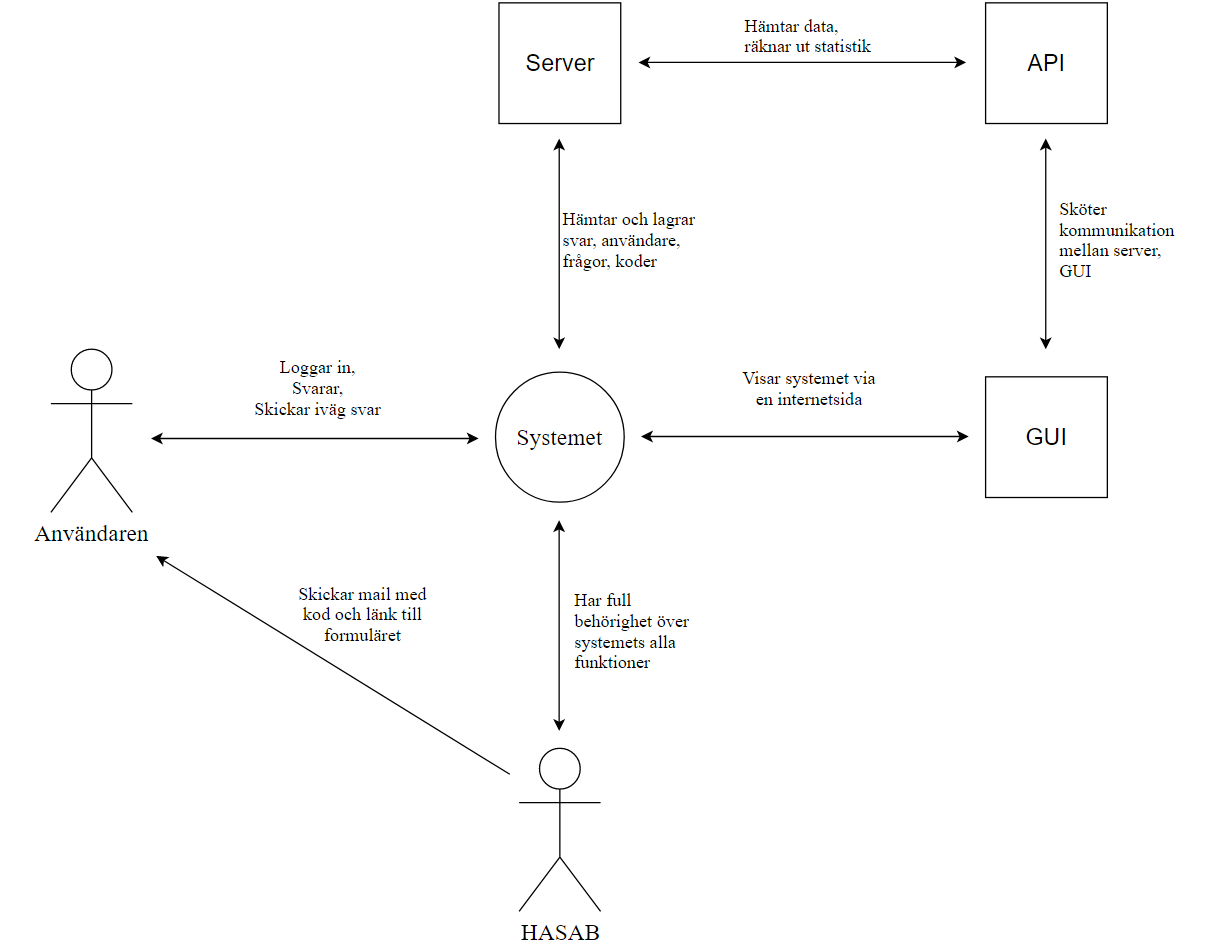
\includegraphics[width=150mm]{Kontextdiagram.png}
    \caption{Kontext-diagram}
    \end{figure}
    
    \newpage
    \subsection{Krav}
    Systemt ska hantera data enligt diagrammet nedan.
       \begin{figure}[h!]
    
    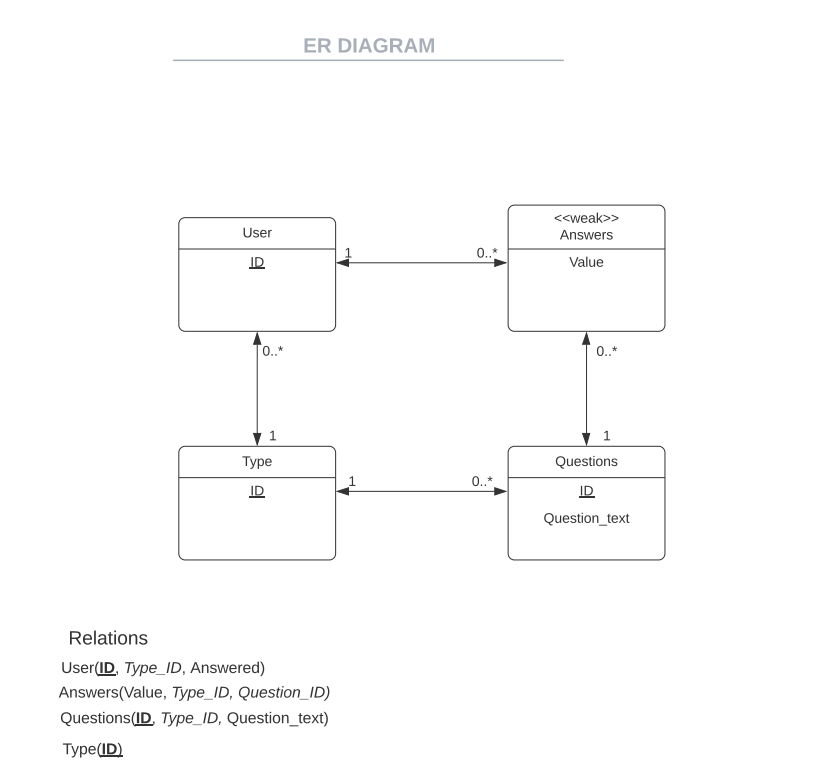
\includegraphics[width=150mm]{ERDIAGRAM.png}
    \caption{ER-Diagram}
    \end{figure}
    
    \newpage
    \subsection{Ändringsbenägna krav}
    \subsection{Uteslutna krav}
    
  
   
    \section{Kvalitetskrav}
    \subsection{Stabila krav}
  
     \subsection{Ändringsbenägna krav}
     
     \subsubsection{Krav}
    Systemet ska ha en svarstid på max ... sekunder.
    
    \subsubsection{Krav}
    Rapportering i systemet ska endast kunna göras av en användare som har fått tillgång till hemsidan via mail eller av admin.
    
     \subsubsection{Krav}
    ../.. användare ska kunna besvara enkäten inom ..minuter.
    
    \subsubsection{Krav}
    ../.. användare ska anse att enkäten var lätt att svara på.
    
    \subsection{Uteslutna krav}
\bibliographystyle{alpha}


\end{document}